\section{Results}
\label{sec:results}

\subsection{Weakest-Link Dominance at \texorpdfstring{$K{=}3$}{K=3}}
\label{sec:dominance}

Table~\ref{tab:dominance} reports the log-log OLS regression (Equation~\ref{eq:regression}) for all 12 conditions across the 455 panels ($K{=}3$, 15 judges from Table~\ref{tab:models}).

\begin{table}[t]
\centering
\small
\begin{tabular}{llccc}
\toprule
\textbf{Bench.} & \textbf{Attack} & $\boldsymbol{\eta_{\max}}$ & $\boldsymbol{K_{\mathrm{eff}}}$ & \textbf{Dom.} \\
\midrule
MMLU & Prompt inj.    & $+^{*}$ & $+^{*}$ & Co \\
MMLU & Sycophancy     & $+^{*}$ & $+^{*}$ & Co \\
MMLU & Score manip.   & n.s.    & $+^{*}$ & $K$ \\
MMLU & Verbosity      & $+^{*}$ & $+^{*}$ & Co \\
MMLU & Position bias  & $+^{*}$ & $+^{*}$ & Co \\
MMLU & Authority bias & $+^{*}$ & $+^{*}$ & Co \\
\addlinespace
ARC  & Prompt inj.    & $+^{*}$ & $+^{*}$ & Co \\
ARC  & Sycophancy     & $+^{*}$ & $+^{*}$ & Co \\
ARC  & Score manip.   & $+^{*}$ & $+^{*}$ & Co \\
ARC  & Verbosity      & $+^{*}$ & $+^{*}$ & Co \\
ARC  & Position bias  & n.s.    & $+^{*}$ & $K$ \\
ARC  & Authority bias & $+^{*}$ & $+^{*}$ & Co \\
\bottomrule
\end{tabular}
\caption{Standardized regression coefficients for $\eta_{\max}$ and $K_{\mathrm{eff}}$ across 12 conditions (455 panels, log-log OLS). $+^{*}$/$-^{*}$: FDR-significant positive/negative (Benjamini--Hochberg, $q < 0.05$); n.s.: not significant. Dom.\ column: $\eta$ = $\eta_{\max}$ sole dominant, $K$ = $K_{\mathrm{eff}}$ sole dominant, Co = co-dominant \citep{budescu1993dominance}.}
\label{tab:dominance}
\end{table}

Under OLS, $K_{\mathrm{eff}}$ is positive and FDR-significant in all 12/12 conditions. $\eta_{\max}$ is significant in 10/12 (exceptions: MMLU $\times$ score manipulation and ARC $\times$ position bias), consistent with Theorem~\ref{thm:monotonicity}. Dominance analysis yields 10 co-dominant, 2 $K_{\mathrm{eff}}$-dominant, and zero $\eta_{\max}$-dominant conditions. However, the $r = 0.70$ $K_{\mathrm{eff}}$--$\eta_{\max}$ correlation raises confound concerns, and OLS ignores the non-independence of the 455 panels. The distribution of $K_{\mathrm{eff}}$ across panel sizes is reported in Appendix~\ref{app:keff_dist} (Table~\ref{tab:keff_dist}).

Each judge appears in $\binom{14}{2} = 91$ of the 455 panels, and each pair co-occurs in 13. This shared structure causes OLS to underestimate standard errors by approximately $2.5{\times}$. Figure~\ref{fig:robustness} compares OLS against three corrections: both predictors attenuate under bootstrap ($\eta_{\max}$ 3/12, $K_{\mathrm{eff}}$ 4/12), with $K_{\mathrm{eff}}$ slightly ahead. Point estimates remain positive in all 12 conditions for $K_{\mathrm{eff}}$, but clustered SE confidence intervals are wide at this panel size ($K_{\mathrm{eff}}$ 0/12 significant; Appendix~\ref{app:forest_plot}).

\begin{table}[t]
\centering
\small
\begin{tabular}{lcc}
\toprule
\textbf{Method} & $\boldsymbol{\eta_{\max}}$ \textbf{sig} & $\boldsymbol{K_{\mathrm{eff}}}$ \textbf{sig} \\
\midrule
OLS                    & 10/12 & 12/12 \\
Clustered SE           & 4/12  & 0/12  \\
Mixed effects          & 6/12  & 3/12  \\
Wild bootstrap         & 3/12  & 4/12  \\
Frac.\ logit (clust.)  & 6/12  & 9/12  \\
\bottomrule
\end{tabular}
\caption{Inference method sensitivity at $K{=}3$ (455 panels, 12 conditions). $K_{\mathrm{eff}}$ significance ranges from 0/12 (clustered SE) to 12/12 (OLS), demonstrating that the $K{=}3$ pattern is method-sensitive. All five methods preserve the positive coefficient direction for $K_{\mathrm{eff}}$ (direction 12/12), though significance ranges from 0/12 to 12/12.}
\label{tab:method_comparison}
\end{table}

\begin{figure}[t]
\centering
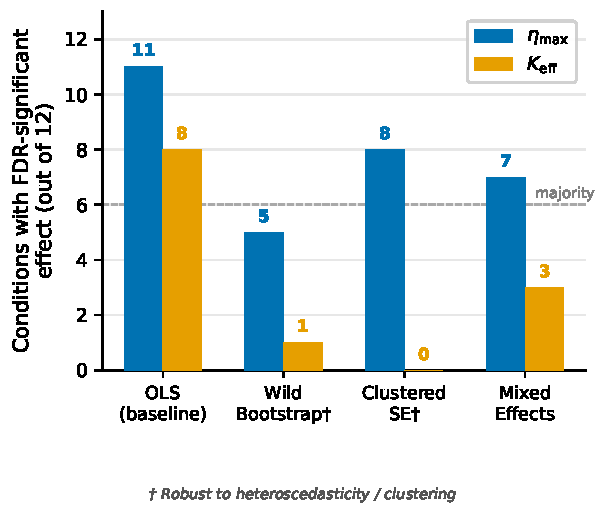
\includegraphics[width=\columnwidth]{figures/fig1_robustness_comparison.pdf}
\caption{Significance counts (FDR $< 0.05$) for $\eta_{\max}$ and $K_{\mathrm{eff}}$ across four correction methods over 12 experimental conditions ($K{=}3$). Wild cluster bootstrap and clustered standard errors are recommended for the 15-judge combinatorial design.}
\label{fig:robustness}
\end{figure}

Power analysis yields MDE $\beta_{\mathrm{std}} = 0.14$ at 80\% power (decreasing to 0.048 at $K{=}5$; Appendix~\ref{app:power_analysis}). The bootstrap attenuation at $K{=}3$ (OLS 12/12 $\to$ bootstrap 4/12) is consistent with this MDE, though positive coefficient direction (12/12) is preserved across all methods despite significance ranging from 0/12 to 12/12. Random subsampling further confirms stability (Appendix~\ref{app:random_subsample}).

\subsection{Panel-Size-Dependent Predictor Shift}
\label{sec:cross_k}

Table~\ref{tab:method_comparison} reveals that the $K{=}3$ pattern is method-sensitive: $K_{\mathrm{eff}}$ significance ranges from 0/12 (clustered SE) to 12/12 (OLS), with fractional logit giving 9/12. This contrasts with $K{\geq}5$, where $K_{\mathrm{eff}}$'s dominance is consistent across all methods (bootstrap 7/12 at $K{=}5$; fractional logit 11/12).

We repeat the wild cluster bootstrap at $K \in \{3, 5, 7\}$, constructing all $\binom{15}{K}$ panels with $K$-position max-$p$ correction.

\begin{figure}[t]
\centering
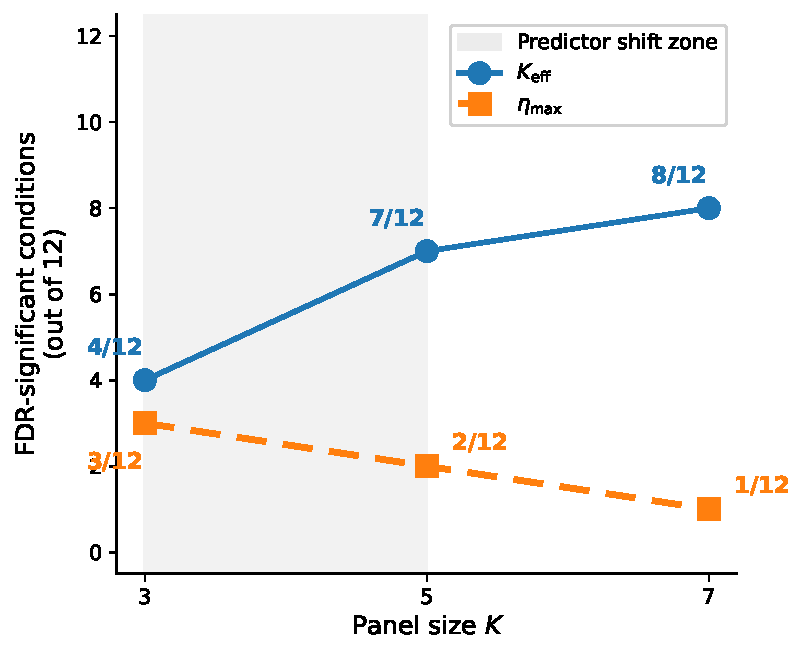
\includegraphics[width=\columnwidth]{figures/fig_regime_transition.pdf}
\caption{Predictor shift across panel sizes. $\eta_{\max}$ significance (orange) declines from 3/12 to 2/12, while $K_{\mathrm{eff}}$ significance (blue) rises from 4/12 to 7/12 as $K$ increases from 3 to 5. Shaded region marks the predictor shift zone $K^* \in (3, 5)$. Bootstrap: $B{=}9999$, Rademacher weights, position-permutation max-$p$, BH FDR $\alpha{=}0.05$.}
\label{fig:regime_transition}
\end{figure}

Figure~\ref{fig:regime_transition} reveals a predictor shift between $K{=}3$ and $K{=}5$. At $K{=}3$, both predictors contribute modestly ($\eta_{\max}$ 3/12, $K_{\mathrm{eff}}$ 4/12)---co-determination. At $K{=}5$, $\eta_{\max}$ drops to 2/12 while $K_{\mathrm{eff}}$ rises to 7/12, all positive. Restricting to the four $K_{\mathrm{eff}}$-stable attacks ($\rho{\geq}0.91$; Appendix~\ref{app:attacked_keff}) confirms that the signal is not driven by measurement-unstable conditions. $K_{\mathrm{eff}}$ significance increases monotonically ($4 \to 7 \to 8$) from $K{=}3$ to $K{=}7$ (\S\ref{sec:analysis}).

\subsection{Random vs.\ Adaptive Fault Contrast}
\label{sec:rf_contrast}

We simulate non-adversarial noise by randomly flipping judge votes at observed per-judge error rates. Random faults yield $R^2 = 0.73$--$0.81$ ($K_{\mathrm{eff}}$ significant 2/2); adaptive attack reduces predictability ($R^2{=}0.275$ at $K{=}5$) but $K_{\mathrm{eff}}$ retains power (7/12). The predictability gap narrows from ${\sim}0.6$ ($K{=}3$) to $0.43$ ($K{=}5$).

\subsection{Positive Direction Across Attack Types}
\label{sec:gam_taxonomy}

GAM bootstrap confirms that $K_{\mathrm{eff}}$'s coefficient direction is positive in all 12 conditions (88.9--100\% positive rate at $K{=}3$, 100\% at $K{=}5$; Figure~\ref{fig:gam_split}). A Kruskal--Wallis test finds no significant magnitude difference between targeted and shared-bias attacks ($p{=}0.200$ at $K{=}3$, $p{=}0.423$ at $K{=}5$).

\subsection{Aggregation Rules and the Diversity Channel}
\label{sec:aggregation}

Table~\ref{tab:aggregation} reports regression results for four aggregation methods across all 12 conditions.

\begin{table}[t]
\centering
\small
\begin{tabular}{lcccc}
\toprule
\textbf{Method} & \textbf{$\eta_{\max}$ sig} & \textbf{$K_{\mathrm{eff}}$ sig} & \textbf{$K_{\mathrm{eff}}$ $\beta$ dir.} & \textbf{$R^2$} \\
\midrule
Threshold       & 12/12 & 11/12 & 11+/0$-$  & 0.829 \\
Majority        & 10/12 & 12/12 & 12+/0$-$  & 0.327 \\
Weighted        & 9/12  & 12/12 & 12+/0$-$  & 0.328 \\
Bayesian        & 9/12  & 6/12  & 5+/1$-$   & 0.087 \\
\bottomrule
\end{tabular}
\caption{Aggregation method comparison ($K{=}3$, 15 models, 455 panels, OLS log-log). Significance counts are FDR-corrected across 12 conditions. $R^2$ is the mean across conditions. Table~\ref{tab:dominance} uses per-condition FDR; this table uses pooled FDR across conditions.}
\label{tab:aggregation}
\end{table}


The methods form a predictability gradient from threshold ($R^2{=}0.829$) to Bayesian ($R^2{=}0.087$; Appendix~\ref{app:aggregation_details}). $K_{\mathrm{eff}}$'s positive direction is preserved under majority (12+/0$-$) and weighted (12+/0$-$) voting; Bayesian calibration attenuates $K_{\mathrm{eff}}$ (5+/1$-$) but $\eta_{\max}$ persists (9/12), yielding partial defense.

\paragraph{Fractional Logit Robustness.}
Fractional logit \citep{papke1996econometric} with clustered SE confirms the predictor shift: $K_{\mathrm{eff}}$ significance increases from 9/12 ($K{=}3$) to 11/12 ($K{=}5$) to 12/12 ($K{=}7$), with 98.6\% directional concordance with OLS (71/72; Appendix~\ref{app:robustness_checks}).
